\documentclass[10pt,a4paper]{article}

\usepackage[margin=0.62in]{geometry}
\usepackage{graphicx}
\usepackage{booktabs}
\usepackage{array}
\usepackage{xcolor}
\usepackage{titlesec}
\usepackage{enumitem}
\usepackage{multicol}
\usepackage{tikz}
\usepackage{float}
\usepackage{hyperref}
\usepackage{caption}
\usepackage{fancyhdr}

\usetikzlibrary{arrows.meta, positioning, shapes.geometric}

\definecolor{primary}{HTML}{0B3D2E}
\definecolor{accent}{HTML}{C75B12}
\definecolor{softgray}{HTML}{F4F6F5}

\hypersetup{
    colorlinks=true,
    linkcolor=primary,
    urlcolor=accent
}

\pagestyle{fancy}
\fancyhf{}
\lhead{\textcolor{primary}{Forest Firefighting Robotics Mission}}
\rhead{\textcolor{primary}{Webots + Mavic Drones}}
\cfoot{\thepage}

\titleformat{\section}
  {\large\bfseries\color{primary}}
  {\thesection}{0.5em}{}

\titleformat{\subsection}
  {\normalsize\bfseries\color{accent}}
  {\thesubsection}{0.5em}{}

\setlist[itemize]{leftmargin=1.2em, itemsep=1pt, topsep=2pt}
\setlength{\parindent}{0pt}
\setlength{\parskip}{4pt}

\begin{document}

\begin{center}
    {\Large \textbf{\textcolor{primary}{Autonomous Forest Firefighting Mission using Webots Mavic Drones}}}\\[4pt]
    {\normalsize Undergraduate Robotics Practical Simulation Test}\\[2pt]
    {\small Platform: Webots R2021b Forest Firefighters Project \quad | \quad Controller: Python}\\[6pt]
\end{center}

\vspace{-0.4em}

\section{Introduction}
This project implements an autonomous forest firefighting mission in the Webots Forest Firefighters simulation environment. The mission objective is to use robots to patrol a forest, detect fire or smoke using onboard cameras, navigate toward the detected fire, and extinguish it by dropping water. The final solution uses four Mavic drone controllers deployed across the four forest quadrants, supported by a Spot-like ground robot. This configuration preserves full forest coverage while reducing camera, controller, and overlay load on the NVIDIA RTX A1000 6 GB GPU.

The implementation was executed in a stable Webots R2021b Docker environment with NVIDIA GPU OpenGL rendering. Before each mission test, a preflight checker verified that all four drones started from separate quadrant base positions:
\begin{itemize}
    \item \textbf{SW Quadrant}: Drone 1 at $(4.0, 4.0, 17.4)$
    \item \textbf{NW Quadrant}: Drone 2 at $(2.0, 26.0, 18.82)$
    \item \textbf{SE Quadrant}: Drone 3 at $(26.0, 3.0, 15.25)$
    \item \textbf{NE Quadrant}: Drone 4 at $(28.0, 26.0, 19.34)$
\end{itemize}
This ensured that all later results measured mission behaviour rather than incorrect spawn placement.

\section{System Architecture}
The system is organised as a closed-loop autonomous robotics pipeline. The Webots world provides the terrain, fire propagation, smoke, drone bodies, sensors, and water-drop mechanism. Each Mavic drone uses its camera for perception, GPS for localisation, and IMU/gyro data for stabilised movement.

\begin{figure}[H]
\centering
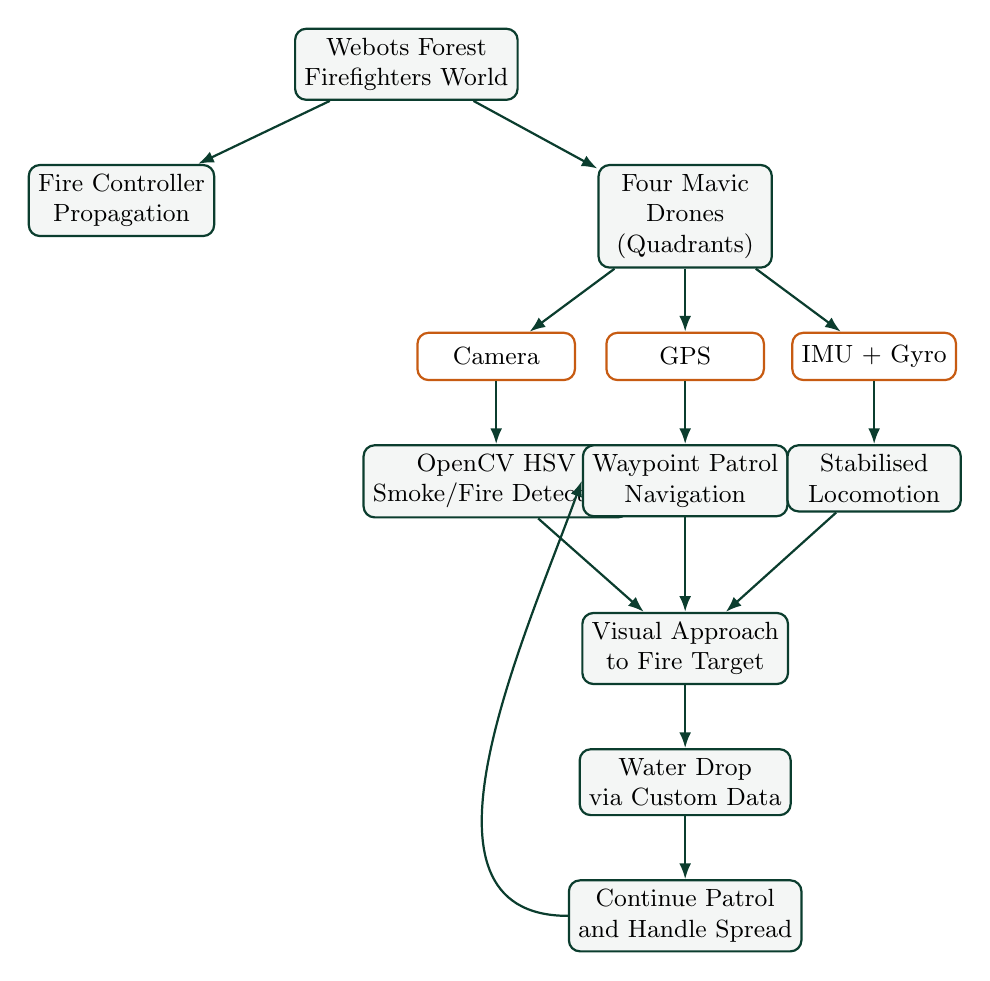
\begin{tikzpicture}[
    node distance=0.8cm and 1.0cm,
    block/.style={rectangle, rounded corners, draw=primary, fill=softgray, thick, align=center, minimum width=2.2cm, minimum height=0.65cm, font=\small},
    sensor/.style={rectangle, rounded corners, draw=accent, fill=white, thick, align=center, minimum width=2.0cm, minimum height=0.6cm, font=\small},
    arrow/.style={-{Latex[length=2mm]}, thick, color=primary}
]
\node[block] (world) {Webots Forest\\Firefighters World};
\node[block, below left=of world] (fire) {Fire Controller\\Propagation};
\node[block, below right=of world] (drones) {Four Mavic\\Drones\\(Quadrants)};

\node[sensor, below=of drones, xshift=-2.4cm] (camera) {Camera};
\node[sensor, below=of drones] (gps) {GPS};
\node[sensor, below=of drones, xshift=2.4cm] (imu) {IMU + Gyro};

\node[block, below=of camera] (detect) {OpenCV HSV\\Smoke/Fire Detection};
\node[block, below=of gps] (nav) {Waypoint Patrol\\Navigation};
\node[block, below=of imu] (stability) {Stabilised\\Locomotion};

\node[block, below=1.2cm of nav] (approach) {Visual Approach\\to Fire Target};
\node[block, below=of approach] (drop) {Water Drop\\via Custom Data};
\node[block, below=of drop] (loop) {Continue Patrol\\and Handle Spread};

\draw[arrow] (world) -- (fire);
\draw[arrow] (world) -- (drones);
\draw[arrow] (drones) -- (camera);
\draw[arrow] (drones) -- (gps);
\draw[arrow] (drones) -- (imu);
\draw[arrow] (camera) -- (detect);
\draw[arrow] (gps) -- (nav);
\draw[arrow] (imu) -- (stability);
\draw[arrow] (detect) -- (approach);
\draw[arrow] (nav) -- (approach);
\draw[arrow] (stability) -- (approach);
\draw[arrow] (approach) -- (drop);
\draw[arrow] (drop) -- (loop);
\draw[arrow] (loop.west) to[out=180,in=250] (nav.west);
\end{tikzpicture}
\caption{System architecture for autonomous aerial firefighting.}
\end{figure}

\vspace{-0.6em}

\newpage
\section{Methodology and Key Algorithms}
\subsection{Locomotion and Stabilisation}
The Mavic drone is controlled using four propeller motors. The controller computes motor velocities from vertical thrust, roll, pitch, yaw, and altitude error. GPS provides position and altitude feedback, while the inertial unit and gyro provide orientation and angular velocity. This supports stable aerial locomotion during takeoff, patrol, fire approach, and hovering over the target.

\subsection{Waypoint Patrol Navigation}
Each drone receives patrol coordinates through controller arguments in the world file. The controller stores these coordinates as a waypoint list. During flight, the drone compares its GPS position with the current target waypoint. When it reaches the waypoint within the precision threshold, it automatically switches to the next target. This implements continuous patrol of the forest area.

\subsection{Camera-Based Fire and Smoke Detection}
The onboard camera captures a downward-facing image. The image is converted into an OpenCV-compatible format and then transformed into HSV colour space. A colour threshold isolates bright low-saturation smoke/fire regions. Contours are extracted from the binary mask, and the largest valid contour is selected as the active fire target. The output is an image coordinate $(x,y)$ used by the approach controller.

\subsection{Fire Approach and Water Drop}
After a fire is detected, the controller compares the detected image coordinate with the centre of the camera frame. If the fire is not centred, yaw and pitch disturbances guide the drone toward it. When the fire is centred below the drone, the controller triggers a water-drop command using the drone custom data field. The drone then clears the current target and continues the patrol loop, allowing it to respond to additional propagated fires.

\section{Performance Results}
Three repeated mission tests were executed after the launch-position preflight check passed. The first repeat was the cleanest run and is used as the primary demonstration result.

\begin{table}[H]
\centering
\caption{Mission performance across repeated tests.}
\small
\begin{tabular}{lrrrrrr}
\toprule
Run & Detections & Drops & Targets & Errors & Crashes & Shutdown Artifacts \\
\midrule
stability\_repeat\_01 & 107 & 5 & 4 & 0 & 0 & 0 \\
stability\_repeat\_02 & 79 & 7 & 4 & 0 & 2 & 3 \\
stability\_repeat\_03 & 59 & 5 & 4 & 0 & 6 & 4 \\
final\_demo\_test & 46 & 4 & 5 & 0 & 0 & 3 \\
\bottomrule
\end{tabular}
\end{table}

The primary run, \texttt{stability\_repeat\_01}, achieved 107 camera-based detections, 5 water drops, 4 waypoint target transitions, and no mission errors or crashes. After identifying and fixing a safe perception bug in the fire detection routine, the final validation test achieved 46 detections, 4 water drops, 5 target transitions, and no mission errors or mission crashes. This confirms that the final controller is stable enough for live demonstration.
\section{Challenges and Solutions}
\begin{table}[H]
\centering
\caption{Key engineering challenges and solutions.}
\small
\begin{tabular}{p{0.43\linewidth} p{0.50\linewidth}}
\toprule
Challenge & Solution \\
\midrule
The fire detection function could crash when smoke was detected but no valid contour was selected. & A safe initialisation fix was added so the function returns an empty list instead of raising an \texttt{UnboundLocalError}. \\
Webots R2025a produced missing PROTOs, broken terrain, and unstable Mavic behaviour. & The project was moved to Webots R2021b, where the Forest Firefighters world runs correctly. \\
Docker initially used software rendering, causing slow simulation. & NVIDIA GPU rendering was enabled and verified using \texttt{glxinfo}. \\
Running Webots as root caused sandbox-related crashes. & A non-root Docker user was created for stable execution. \\
The drones appeared high because of terrain elevation and target altitude values. & A static launch check confirmed correct base spawn positions before testing. \\
Instrumentation changed timing and destabilised flight. & The controller was restored to the stable baseline; external log analysis was used instead. \\
Shutdown warnings appeared in some runs. & The analyzer separated mission performance from Webots/Chromium shutdown artifacts. \\
\bottomrule
\end{tabular}
\end{table}

\section{Conclusion}
The final system demonstrates an autonomous firefighting mission using four Mavic drones deployed across four forest quadrants in Webots, supported by a Spot-like ground robot. The drones patrol their assigned forest quadrants, detect smoke/fire with camera-based OpenCV processing, navigate toward detected fire regions, drop water, and continue patrolling for additional propagated fires. The updated four-drone configuration reduces simulation load while preserving full-area coverage, satisfying the mission requirements for locomotion, perception, navigation, integration, and documentation.

\end{document}
```
